\chapter{Analýza datových zdrojů} \label{chap:data-sources-analysis}
V následující kapitole shrneme výstupy analýzy datových zdrojů pro FEL ČVUT, která je jedním z cílů této části práce. Obecně jsme datové zdroje řešili v kapitole č. \ref{chap:sources}, nyní na tuto kapitolu navážeme a budeme řešit konkrétní příklady. Zdroje budeme dále kategorizovat do různých skupin. Důležité je zmínit, že v této kapitole nepopíšeme přesný způsob využití jednotlivých zdrojů. Spíše popíšeme, v jaké formě jsou data dostupná a jak by mohla být užitečná.\par
\section{Kategorizace datových zdrojů}
Datové zdroje můžeme rozdělit dle různých kritérií. V této sekci shrneme kategorie, které budeme používat v naší práci.
\paragraph{Dle typu obsahu na:}
\begin{itemize}
    \item Osoby a pracoviště
    \item Znalosti
\end{itemize}
\paragraph{Dle typu znalosti (viz kapitola č. \ref{chap:sources}) na:}
\begin{itemize}
    \item Znalostní báze
    \item Osobní znalosti
    \item Obojí
\end{itemize}
\paragraph{Dle příslušnosti datového zdroje na:}
\begin{itemize}
    \item Externí zdroj (případně globální)
    \item Interní zdroj pro danou organizaci - v našem případě pro ČVUT FEL
\end{itemize}

\section{Datové zdroje ČVUT}
% [TODO: obecně ještě zhodnotit ty zdroje, co se týká toho, jak jsou vhodné pro nás]
\subsection{Osoby a pracoviště}
% Co se týká dat o osobách, je důležité zmínit, že můžeme získávat buď jen data veřejně dostupná, nebo je nutné sbírat souhlasy od dotyčných osob.\par
\begin{table}[H]
\begin{ctucolortab}
% \begin{tabular}{|l|l|m{3cm}|l|m{2,75cm}|}
\begin{tabularx}{0.95\linewidth}{l|X|X|X}
\bfseries  & \bfseries Forma dat & \bfseries Dostupnost dat  & \bfseries Správce\\\hline 
    % \hline
    %  & Forma dat & Dostupnost dat & Aktualizováno & Správce \\ \hline
    \textbf{Usermap} & REST API (JSON) & veřejná data o zaměstnancích, po domluvě dostupná & ČVUT spravuje systém, FIT spravuje API \\\hline
    \textbf{UDB} & LDAP (LDIF) & veřejná data o zaměstnancích, po domluvě dostupná & FEL \\
\end{tabularx}
\end{ctucolortab}
	\caption{Tabulka dostupných zdrojů osob a pracovišť FEL (zdroj autor)}
	\label{tab:data-sources-people-fel}
\end{table}

\subsubsection{Usermap}
Usermap je centrální systém ČVUT pro správu identit. Jsou zde uloženy informace o osobách, organizační struktuře, pracovištích a jiné. Databáze Usermap má dvě části - LDAP databáze a přidružená relační databáze \cite{usermap-db}. Databáze Usermap je spravována jednotně na úrovni celé univerzity.\par
\begin{figure}[htbp!]
	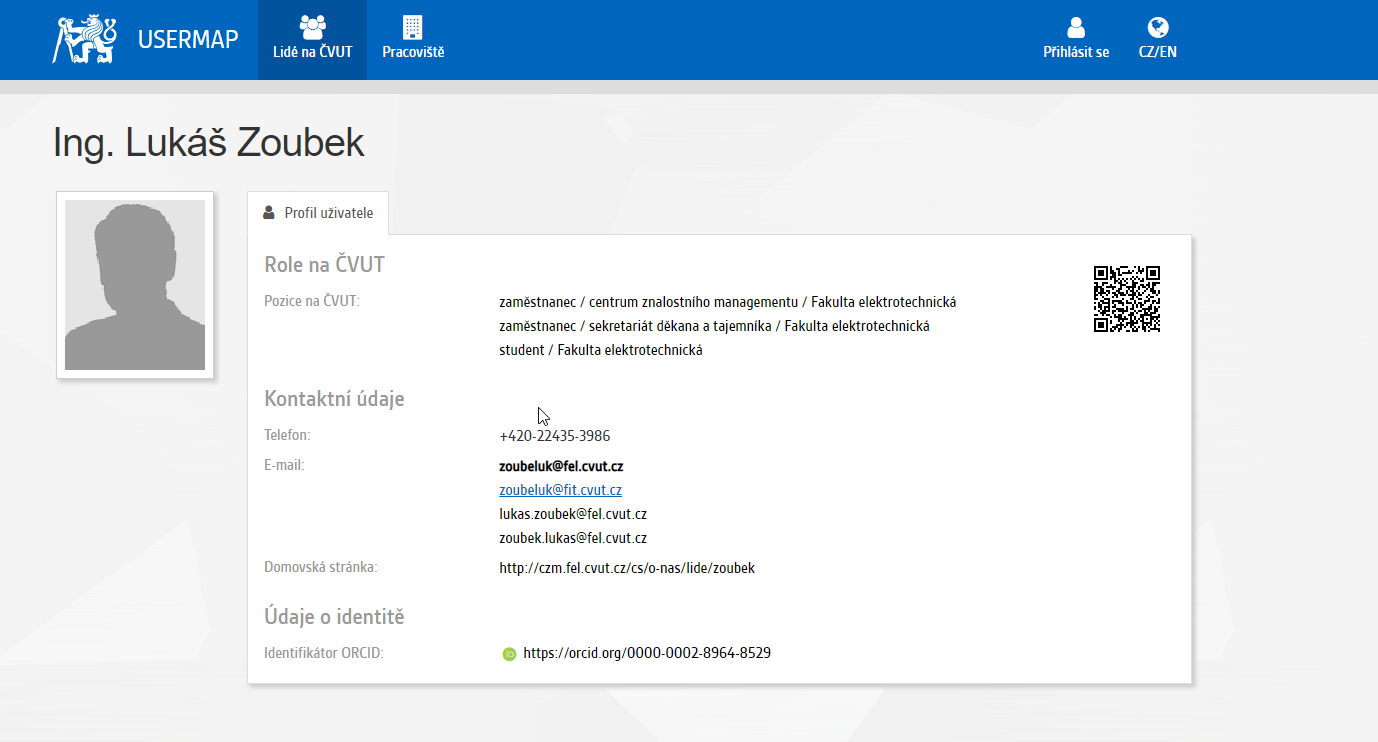
\includegraphics[width=\linewidth]{img/usermap.png}
	\caption{Webové rozhraní systému usermap (Dostupné z:  \url{https://usermap.cvut.cz/search})}
	\label{fig:usermap}
\end{figure}
\noindent REST rozhraní (\textit{Usermap API}) k této databázi je oproti tomu spravováno FIT ČVUT, konkrétně Ing. Jakubem Jirůtkou.
\begin{quote}
 \textit{Usermap API (pracovní název) je agregátor údajů o identitách lidí na ČVUT, který vyvíjíme na FIT. Poskytuje základní informace o osobě jako je jméno, uživatelské jméno, emailové adresy, telefony, … a tzv. byznys role (z IDM). Dále obsahuje informace o organizačních jednotkách ČVUT a místnostech (vč. adresy).} \cite{usermap-api}
\end{quote}
Identifikace v rámci tohoto zdroje probíhá pomocí uid, uživatelského jména v rámci ČVUT. Ve webovém rozhraní aplikace usermap lze též získat ORCID dané osoby - jednoznačný identifikátor vědeckých a dalších akademických autorů\cite{orcid}.
\subsubsection{UDB}
Narozdíl od systému usermap systém UDB je spravován fakultou FEL. Typy obsahu jsou ve své podstatě totožné, nicméně v UDB se nacházejí některá data navíc (fakultního charakteru). K systému neexistuje žádná veřejně dostupná dokumentace.
\subsection{Znalosti}
Již v kapitole č. \ref{chap:sources} jsme zmínili, že jeden fyzický zdroj může být jak zdrojem osobních znalostí, tak zdrojem znalostní báze. V této kapitole jsme se pokusili tyto dvě kategorie od sebe oddělit, nicméně se dá předpokládat, že zdroj nemusí mít vždy jedno diskrétní využití.
\subsubsection{Osobní znalosti}
\begin{table}[h!]
\begin{ctucolortab}
\begin{tabularx}{0.95\linewidth}{l|X|X|X}
\bfseries  & \bfseries Forma dat & \bfseries Dostupnost dat  & \bfseries Správce\\\hline 
    \textbf{V3S} & REST API (XML) & veřejná část & ČVUT spravuje systém, FIT spravuje API \\ \hline
    \textbf{KOS} & REST API (XML) & veřejná část & ČVUT spravuje systém, FIT spravuje API
\end{tabularx}
\end{ctucolortab}
	\caption{Tabulka dostupných zdrojů osobních znalostí na ČVUT (zdroj autor)}
	\label{tab:data-sources-people-fel}
\end{table}
\paragraph{Systém V3S:} V naší práci, jak jsme zmínili již v úvodu, se zabýváme více formálními zdroji znalostí (např. vědecké články, patenty). Předpokládáme, že systém V3S je pro data tohoto typu klíčový. Pokud bychom řešení opřeli o tento systém, množinu vyhledávaných bychom omezili na ty, kteří jsou vědecky aktivní. Má tedy smysl se zabývat i ostatními zdroji.\par
Aplikace V3S obsahuje záznamy o veškeré vědecké činnosti na univerzitě. Záznamy obsahují metadata o publikovaných článcích, autorech a dalších souvisejících entitách. Plné texty některých článků jsou k dispozici v digitální knihovně ČVUT (Dspace - https://dspace.cvut.cz/\url{https://dspace.cvut.cz/}). Nejedná se však o všechny články, ne všechny může ČVUT takto ukládat a poskytovat.\par
\noindent REST rozhraní \textit{V3S API} k této databázi je spravováno FIT ČVUT, konkrétně Ing. Jakubem Jirůtkou.\par
\paragraph{KOS (Komponenta studia):} KOS je centrálním informačním systémem pro podporu výuky na ČVUT. Studenti ČVUT přistupují do tohoto systému pomocí webového rozhraní, které obsahuje pouze zlomek dat, které jsou ve skutečnosti v systému k dispozici (v jeho databázi). REST rozhraní \textit{KOS API} k této databázi je správováno FIT ČVUT, konkrétně Ing. Jakubem Jirůtkou.\par
 KOS by mohl být potenciálně zdrojem obsahu jako: studované a vyučované předměty, vedené a nabízené závěrečné práce.\par
\paragraph{Ostatní:} Pracovníci FEL ČVUT mohou sami sloužit jako zdroj jejich znalostí - jejich životopisy, osobní stránky a jiné. Tyto zdroje typicky postrádají jakoukoliv jednotnou strukturu či rozhraní, jsou tedy špatně strojově zpracovatelné.
 \begin{figure}[htbp!]
	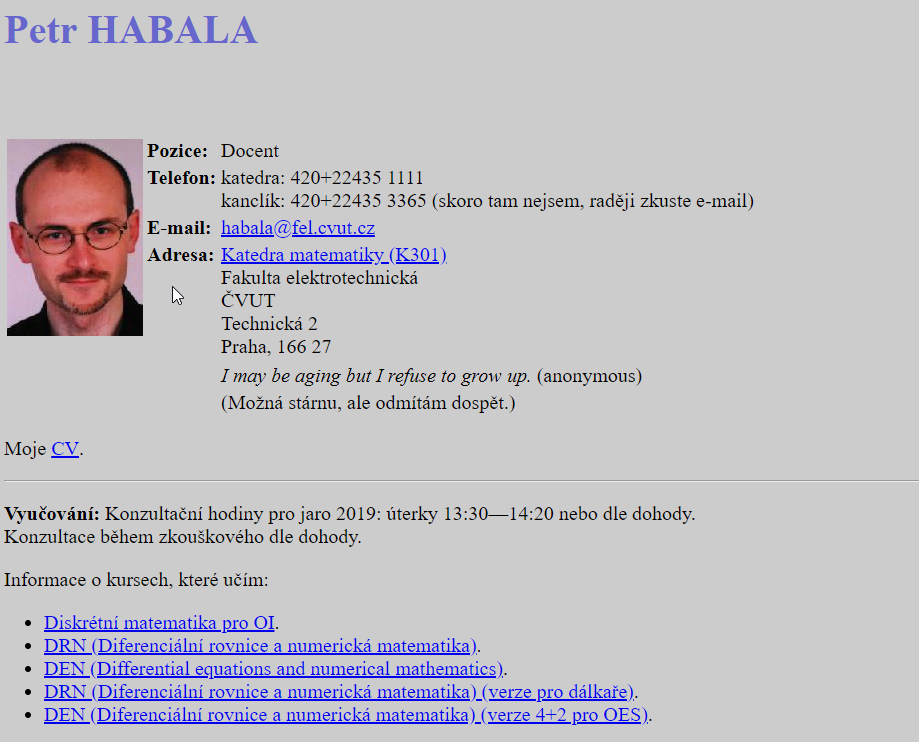
\includegraphics[width=\linewidth]{img/personal-pages.png}
	\caption{Webové stránky pracovníka katedry matematiky, docenta Habaly (Dostupné z:  \url{https://math.feld.cvut.cz/habala/indexc.htm})}
	\label{fig:personal-pages}
\end{figure}
 Při rešerši možných zdrojů jsme narazili ještě na systém DNEP (databáze nabídek, expertů a přístrojů), který nejspíše spravuje ČVUT. Systém obsahuje expertů pouze 93 (zjištěno z aplikace), na základě tohoto faktu jsme konstatovali, že není dále aktualizován a používán.

\subsubsection{Znalostní báze}
Potenciálně využitelným zdrojem znalostní báze přímo na ČVUT by mohl být systém V3S potažmo digitální knihovna DSpace. Data v těchto zdrojích (hlavně texty) by se po anotaci \cite{semantic-annotation} mohla použít při plnění ontologií, slovníků a jiných.\par 
Sémantická anotace textu je jednou z možných technik pro obohacování textu o význam, což je při tvorbě znalostní báze dosti klíčové. Sémantická anotace textu není triviální činnost, ruční provedení může trvat velmi dlouho a semi-automatické či automatické necháme na budoucí práci (zabývají se jí například nástroje jako je Tagtog - dostupné z: \url{https://www.tagtog.net/}, nebo LightTag dostupné z: \url{https://www.lighttag.io/}).

\section{Externí (globální) datové zdroje}
Při získávání informací o osobách a pracovištích jsme odkázáni na interní zdroje, externí zdroje můžeme použít pro znalosti. 
\subsection{Znalosti}
\subsubsection{Osobní znalosti}
Systém V3S považujeme za nejdůležitější a nejobjektivnější zdroj znalostí vědeckých pracovníků FEL. Další podobné zdroje jsou zmíněny v této sekci, jedná se však již o systémy, které nejsou ve správě fakulty/univerzity.
%  Jak jsme již zmínili v úvodu této sekce a v sekci zabývající se systémem V3S, nejkvalitnější data týkající se znalostí jsou pro nás výstupy vědecké činnosti. 
 %Dalšími potenciálními zdroji by pochopitelně mohli být některé veřejně dostupné informace např. sociální sítě aj., ty jsme však v této práci vynechali, soustředíme se více na oficiální zdroje. 
\begin{table}[h!]
\begin{ctucolortab}
\begin{tabularx}{0.95\linewidth}{X|p{5cm}|X}
\bfseries  & \bfseries Forma dat &  \bfseries Správce\\\hline 
    \textbf{Scholar, google patenty} & oficiální API chybí & Google\\ \hline
    \textbf{Scopus} & REST API (různé formáty) & Elsevier B.V. \\ \hline
    \textbf{Science Direct} & REST API (různé formáty, též fulltext search) & Elsevier B.V.\\ \hline
    \textbf{Springer} & REST API (různé formáty & Springer Nature \\ \hline
    \textbf{IEEE explore} & REST API (různé formáty) & IEEE \\ \hline
    \textbf{Web of Science} & REST API (různé formáty) & Clarivate Analytics \\ \hline
    \textbf{IS výzkumu, experimentálního vývoje a inovací} & API \cite{rvvi} & Úřad vlády České republiky \\ \hline
\end{tabularx}
\end{ctucolortab}
	\caption{Tabulka některých veřejně dostupných zdrojů osobních znalostní (zdroj autor)}
	\label{tab:data-sources-public}
\end{table}

 V rámci veřejných rozhraní je třeba vyřešit identifikaci osob z FEL ČVUT. Vzhledem ke zdrojům které máme k dispozici, se zaměřujeme nejvíce na vědecky aktivní část FEL ČVUT. Existují různé způsoby, jak identifikovat vědce či vědkyně.\par
 \paragraph{Příklady identifikátorů:}
 \begin{itemize}
     \item ORCID - Open Research and Contributor ID (neproprietární)
     \item RID - ResearcherID (proprietární Web of Science)
     \item Scopus Author ID (proprietární Scopus)
 \end{itemize}

\subsubsection{Znalostní báze}
% [TODO: možná zmínit, co od takového zdroje očekáváme]
Je důležité zmínit, že množství dostupných strukturovaných dat, které lze považovat za znalosti, je omezené. Existující datové množiny jsou mezi sebou provázány. Nejčastějšími primárními zdroji jsou Wordnet a Wikipedia (případně její strojově lépe čitelná verze DBPedia). Navazující projekty s těmito zdroji pracují a přidávají další, často užitečné, informace (aktivní přispívání znalostí však často neprobíhá).\par
\noindent Na základě tohoto kritéria datové zdroje rozdělíme do dvou skupin:
\begin{itemize}
    \item Primární zdroje - DBPedia, Wordnet
    \item Agregátory a procesory znalostí - ConceptNet, Yago, Datamuse, Twinword API, WordsAPI
\end{itemize}
% Uvádíme pouze příklady datových zdrojů znalostní báze. Další dostupné zdroje mohou být dostupné například u velkých poskytovatelů jako je Google (dostupné na: \url{https://console.cloud.google.com/apis}) aj.

\paragraph{DBpedia:}
DBpedia extrahuje informace z Wikipedie a následně data propojuje s ostatními získanými daty. Tímto způsobem vzniká jednotná znalostní báze \cite{db-pedia-article}. Tato znalostní báze je dostupná buď ve formě RDF s definovaným OWL schématem ke stažení, přes SPARQL rozhraní nebo též přes webové REST rozhraní \cite{db-pedia-web}. V roce 2014 měla DBpedia 3 miliardy RDF triplů. \cite{db-pedia-web}
\begin{figure}[htbp!]
	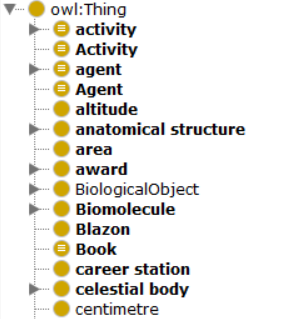
\includegraphics[width=0.45\linewidth]{img/db-pedia.png}
	\caption{Část ze schématu DBpedia v programu Protégé \url{https://protege.stanford.edu/} (zdroj autor)}
	\label{fig:dbpedia}
\end{figure}
\paragraph{WordNet:}
Dalším významným datovým setem je Wordnet. Jedná se o rozsáhlou lexikální databázi anglického jazyka. Slova jsou seskupována do množin synonym. Tyto množiny jsou později propojeny do sítí na základě významových a lexikálních vztahů. Wordnet neřeší slova pouze jako množinu znaků, orientuje se na jejich význam a pracuje například s podobností významu různých slov. \cite{princeton-wordnet} \par
\noindent Data jsou dostupná volně ke stažení, případně přes REST API \cite{princeton-wordnet}.
\paragraph{Agregátory a procesory:} \par
ConceptNet je volně dostupná sémantická síť čerpající mimo jiné z projektů DBpedia a Wordnet. Jedním ze zdrojů dat byla též komunita lidí, projekt Open Mind Common Sense. ConceptNet má API s výstupním formátem JSON-LD. \cite{ConceptNet} 
% [možná odcitovat ještě stránky, ten paper je odkazován na stránkách, ale nevím, co v něm je]
\par
Yago je rozsáhlá sémantická znalostní báze, která čerpá mimo jiné z Wikipedie a Wordnetu. Yago má více než 10 milionů entit. \cite{yago} Yago ontologie je k dispozici ke stažení, například ve formátu TURTLE. Software Yago je k dispozici ve formě zdrojového kódu též volně ke stažení.\cite{yago-web}\par
Dalšími datovými zdroji spadajícími do této kategorie mohou být například Datamuse \cite{datamuse}, Twinword API \cite{twinword} nebo Words API \cite{words-api}. Funkce, kterými disponují jsou typicky hledání slov s podobným významem, hledání slov souvisejících, hledání definic, lematizace (postup převádějící slova na základní gramatický tvar). \par
\section{Shrnutí}
V této kapitole jsme se zabývali rešerší datových zdrojů na FEL ČVUT, tím jsme navázali na kapitolu \ref{chap:sources}, kde jsme tuto problematiku řešili obecně.\par
Datové zdroje jsme rozdělili do kategorií a u každého jsme zmínili důležité parametry. Tím jsme naplnili jeden z cílů této práce.

% [TODO: obecný úvod - co je to za zdroje, co poskytují]


% \begin{table}[h!]
% \begin{tabular}{|m{3cm}|l|m{3cm}|l|m{2,75cm}|}
%     \hline
%     \cellcolor[HTML]{FFFFFF} & Forma dat & Správce \\ \hline
%     \textbf{CoceptNet} & oficiální API chybí & Google\\ \hline
%     \textbf{DBpedia} & REST API (různé formáty) & Elsevier B.V. \\ \hline
%     \textbf{Yago} & REST API (různé formáty, též fulltext search) & Elsevier B.V.\\ \hline
%     \textbf{WordNet} & REST API (různé formáty & Springer Nature \\ \hline
%     \textbf{Google data} & REST API (různé formáty) & IEEE \\ \hline
%     \textbf{Graphwords} & REST API (různé formáty) & Clarivate Analytics \\ \hline
%     \textbf{Datamuse} & API \cite{rvvi} & Úřad vlády České republiky \\ \hline
%     \textbf{Twinword} & API \cite{rvvi} & Úřad vlády České republiky \\ \hline
%     \textbf{Wordapi} & API \cite{rvvi} & Úřad vlády České republiky \\ \hline
% \end{tabular}
% 	\caption{Tabulka některých veřejně dostupných zdrojů znalostní báze (zdroj autor)}
% 	\label{tab:data-sources-public-knowledge.base}
% \end{table}


% %  - https://aleph.nkp.cz/F/DST1KFNIRM63S8U5SV5FJ9CF73L4H7PL9CR7Q4RUYBAKXG85BK-30094?func=file&file_name=find-b
% CoceptNet - http://conceptnet.io/
% DBpedia - https://wiki.dbpedia.org/
% Yago - https://datahub.io/collections/yago
% WordNet - https://wordnet.princeton.edu/ (případně jiné slovníky - Collins, https://onelook.com, Oxford, Wordnik, )
% google.com - translator
% https://graphwords.com/word#wood
% % https://en.wiktionary.org/wiki/deep_learning#English
% http://www.wiksearch.com/?s=buttock
% http://www.datamuse.com/api/
% https://www.twinword.com
% https://www.wordsapi.com


%  [Potenciálně do této kapitoly dodat tabulku s přehledným srovnáním aplikací, potenciálně jejich srovnání v rámci vlastností dobrých datových zdrojů pro ontologické zpracování]

 
 
 
 







%  \section{Datové zdroje dostupné pro ČVUT FEL}
%  Datové typy, které jsou potřeba pro tvorbu databáze znalostí jsou: \textit{Osoby, pracoviště a znalosti}. Tyto entity lze v každé organizaci získat různými způsoby. V kapitole o obecných datových zdrojích [TODO: odkaz] jsme konstatovali, že \textit{Osoby a pracoviště} jsme schopni získat poměrně přímočarým způsobem. \textit{Znalosti} jsou na rozdíl od těchto dvou entit velmi komplikovaným datovým typem. V sekci [TODO: odkaz], o reprezentaci dat, jsme rozebrali různé způsoby, jak znalosti reprezentovat. V závěru jsme se rozhodli, že nejvýhodnější bude použít reprezentaci pomocí ontologií. V dalších sekcích [TODO: sekce odkaz] jsme řešili, v jaké podobě jsou většinou data dostupná (XML, JSON) a do jaké podoby je chceme dostat (jakýkoliv typ serializace RDF - RDF XML, JSON LD, Turtle).\par


% \par
%  Důležité je brát v úvahu, že znalosti jsou velmi abstraktní pojem, i přesto že jsme si zvolili formu jejich reprezentace. V této sekci zmíníme i zdroje, které nejsou aktuálně uchopitelné pro přímou transformaci do ontologického schematu. Momentálně je takových zdrojů většina, protože FEL ČVUT neudržuje anotovaná dat na tak vysoké úrovni. Často tedy budeme zmiňovat zdroje, které momentálně nelze vzít, tak jak jsou, a přetransformovat do ontologického schematu.
%  \subsection{Znalosti vázané na osoby FEL ČVUT}
%  Takový datový zdroj musí znalost (v libovolné formě) poskytovat i s vlastníkem. Jinými slovy se jedná o zdroje, kde vlastník figuruje v libovolné spojitosti s entitou, kterou budeme považovat za znalost (resp. budeme počítat, že půjde vhodným definovaným způsobem transformovat na znalost). Zároveň musí takový zdroj vracet sílu znalosti v rámci daného datového zdroje (TODO: odkaz na data-processing), což je atribut vazby mezi znalostí a vlastníkem (TODO: odkaz na diagram, možná ještě nakreslit obrázek sem ve větším detailu, který shrnuje ten úvod celé té kapitoly).\par


%  -	Usermap
% o	Lidé a role, pracoviště
% o	https://kosapi.fit.cvut.cz/usermap/doc/rest-api-v1.html#
% o	Měl bych mít přístup ke všemu – read.

% -	https://udb.fel.cvut.cz/
% o	Po přihlášení!
% o	Vyhledávání dle username, jméno, příjmení
% o	Vyhledávání pracovišť